\documentclass[border={0.5cm 0.5cm 0.5cm 0.5cm}]{standalone}  %E,S,W,N

\usepackage{amssymb}
\usepackage{amsmath}
\usepackage{tikz}
\usetikzlibrary{calc}	%for centerarc
\usetikzlibrary{decorations.text, arrows, arrows.meta,decorations.markings}	%for bendy text

\def\centerarc[#1](#2)(#3:#4:#5)% Syntax: [draw options] (center) (initial angle:final angle:radius)
{ \draw[#1] ($(#2)+({#5*cos(#3)},{#5*sin(#3)})$) arc (#3:#4:#5); }

\begin{document}
	
	%\begin{figure}
	%	\centering
	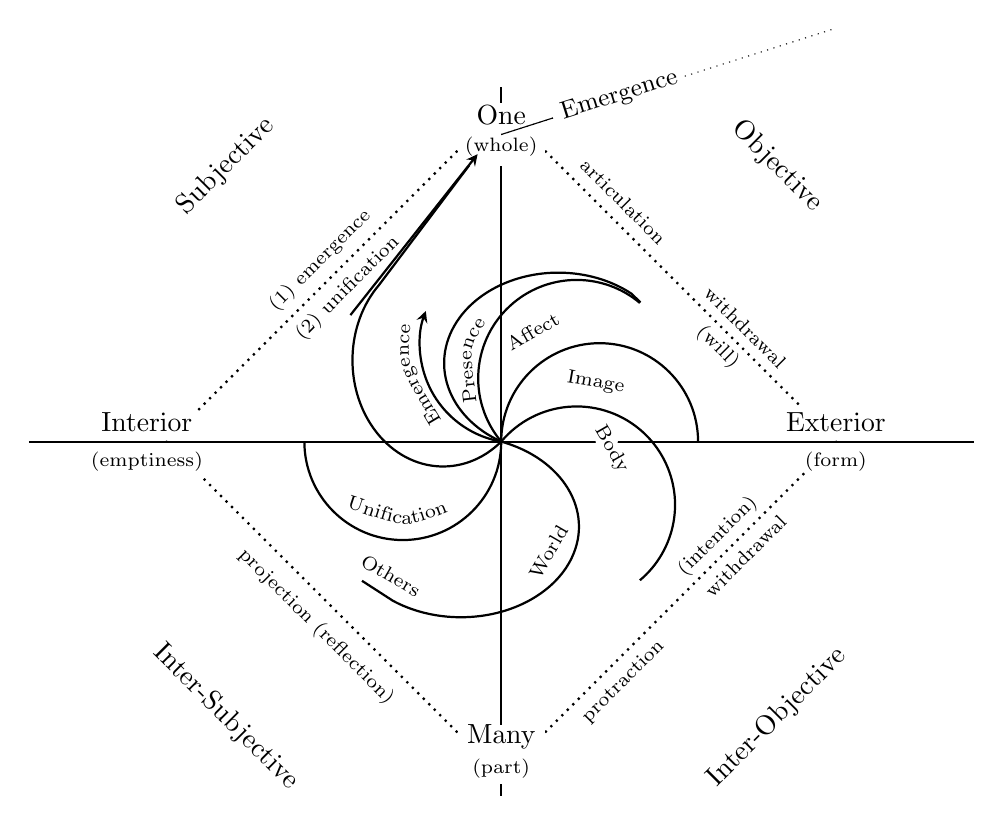
\begin{tikzpicture}
	%AXIS
	\draw[thick] (-6,0)--(6,0);		%x-axis
	\draw[thick] (0,-4.5)--(0,4.5);	%y-axis
	\draw[thick,dotted] (0,-4.25)--( 4.25,0);
	\draw[thick,dotted] (0, 4.25)--( 4.25,0);
	\draw[thick,dotted] (0,-4.25)--(-4.25,0);
	\draw[thick,dotted] (0, 4.25)--(-4.25,0);
	
	%ARCS								%polar coordinates: r*cos(deg), r*sin(deg)
	%\draw[gray] (0,0) circle (2.5);
	%\draw[blue] (0,0)--({2.5*cos(135)},{2.5*sin(135)});
	\centerarc[thick](0,0)(45:-220:2.5)		%upper arrows are at end of code
	%
	\draw[thick,->,>=stealth] (0,0) arc (260:160:1.25cm);
		\draw [decorate, decoration={text along path, text align=center, text={|\scriptsize|Emergencexx}}] (-0.9,0.5) .. controls (-1.2,1) .. (-1.15,1.5);
	\draw[thick] (0,0) arc (240:50:1.45cm and 1.15cm) -- ({2.5*cos(45)},{2.5*sin(45)});
		\draw [decorate, decoration={text along path, text align=center, text={|\scriptsize|Presencexx}}] (-0.35,0.8) .. controls (-0.4,1.2) .. (-0.2,1.5);
	\draw[thick] (0,0) arc (220:50:1.25cm);
		\node at (0.4,1.4) {\rotatebox{30}{\scriptsize Affect}};
	\draw[thick] (0,0) arc (180:0:1.25cm);
		\node at (1.2,0.75) {\rotatebox{-10}{\scriptsize Image}};
	\draw[thick] (0,0) arc (140:-50:1.25cm);
		\fill[white] (1.34,0) circle (4pt);
		\node at (1.4,-0.1) {\rotatebox{-60}{\scriptsize Body}};
	\draw[thick] (0,0) arc (70:-125:1.5cm and 1.15cm) -- ({2.5*cos(-135)},{2.5*sin(-135)});
		\node at (0.6,-1.4) {\rotatebox{60}{\scriptsize World}};
		\node at (-1.4,-1.7) {\rotatebox{-30}{\scriptsize Others}};
	\draw[thick] (0,0) arc (0:-180:1.25cm);
		\draw [decorate, decoration={text along path, text align=center, text={|\scriptsize|Unificationx}}] (-1.8,-0.9) .. controls (-1.2,-1.1) .. (-0.7,-0.9);
	\draw[thick] (0,0) arc (-50:-225:1.15cm and 1.35cm) -- (-0.3,3.65);
	
	%LABELS
	\fill[white] (-0.55,4.3) rectangle (0.55,3.5);
	\node at (0,4.15) {One};
	\node at (0,3.75) {\scriptsize (whole)};
		\draw[dotted] (0,3.9)--(4.25,5.25);
		\draw (0,3.9)--(1.5,4.38);
		\fill[white] (0.6,4.35)--(0.7,3.95)--(2.35,4.5)--(2.25,4.9)--cycle;
		\node at (1.5,4.4) {\rotatebox{17.5}{\small Emergence}};
	%
	\fill[white] (-0.55,-4.35) rectangle (0.55,-3.6);
	\node at (0,-3.75) {Many};
	\node at (0,-4.15) {\scriptsize (part)};
	%
	\fill[white] (-4.5,0.02) rectangle (-3.75,0.38);	%top
	\fill[white] (-4.5,-0.02) rectangle (-3.75,-0.45);	%bottom
	\node at (-4.5,0.25) {Interior};
	\node at (-4.5,-0.25) {\scriptsize (emptiness)};
	%
	\fill[white] (4.5,0.02) rectangle (3.75,0.45);		%top
	\fill[white] (4.5,-0.02) rectangle (3.75,-0.38);	%bottom
	\node at (4.25,0.25) {Exterior};
	\node at (4.25,-0.25) {\scriptsize (form)};
	
	\node at (-3.5, 3.5) {\rotatebox{45}{Subjective}};
	\node at ( 3.5, 3.5) {\rotatebox{-45}{Objective}};
	\node at (-3.5,-3.5) {\rotatebox{-45}{Inter-Subjective}};
	\node at ( 3.5,-3.5) {\rotatebox{45}{Inter-Objective}};
	%
	\node at (-2.3,2.3) {\rotatebox{45}{\scriptsize (1) emergence}};
	\node at (-1.95,1.95) {\rotatebox{45}{\scriptsize (2) unification}};
	%
	\node at (1.55,3.05) {\rotatebox{-45}{\scriptsize articulation}};
	\node at (3.1,1.45) {\rotatebox{-45}{\scriptsize withdrawal}};
	\node at (2.75,1.2) {\rotatebox{-45}{\scriptsize (will)}};
	%
	\node at (1.55,-3.05) {\rotatebox{45}{\scriptsize protraction}};
	\node at (3.1,-1.45) {\rotatebox{45}{\scriptsize withdrawal}};
	\node at (2.75,-1.2) {\rotatebox{45}{\scriptsize (intention)}};
	%
	\node at (-2.35,-2.35) {\rotatebox{-45}{\scriptsize projection (reflection)}};
	
	%ARROW ON ARC
	\draw[thick,->,>=stealth] ({2.5*cos(140)},{2.5*sin(140)})--(-0.3,3.65);
	\end{tikzpicture}
	%	\caption{...}
	%\end{figure}
	
\end{document}